
%\section*{Foreword}
%\begin{figure}[ht] 
%	
%	\centering
%	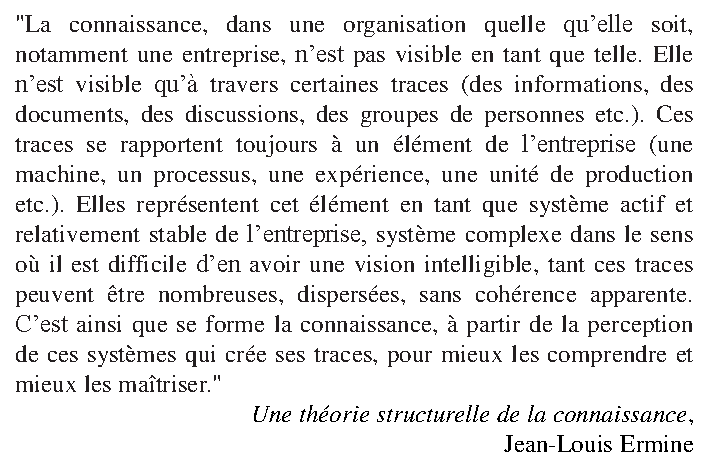
\includegraphics[width=.7\linewidth]{images/citation-ermine.pdf}
%\end{figure}



\section{Introduction}\label{sect:intro}
\sideboxbegin{o}
This document features a protocol to evaluate and extend solutions to traceability (\textit{tracers}). It shows how to integrate trace quality properties, the bottlenecks of the process and its impact on the code. An application onto a specific case shows its usability and provide a first tracer with trace quality for MSBE.
\sideboxend


This report documents the work done as part of the third task described in the Convention de l’équipe de recherche commune. It corresponds to Deliverable 3. The core contribution is an evaluation protocol for solutions to traceability (or \textit{tracers}) and its specific application to an existing solution: Capra\footnote{\url{https://projects.eclipse.org/projects/modeling.capra}}. The protocol features the evaluation of tracers together with the integration of quality concerns for traceability artefacts. 

The two first deliverables of the Trace\textit{a} project constitute the conceptual basis behind this work. The first deliverable, a survey-driven feature model for traceability, shows the general absence of consideration toward trace quality in existing approaches \cite{deliverable1}. The second deliverable presents Trace\textit{a}, our modular metamodel for traceability \cite{deliverable2}. The complete Trace\textit{a} metamodel is available in a paper we submitted to the international working conference on Exploring Modeling Methods for Systems Analysis and Development (EMMSAD 2021) and available on the Modelia's Git repository \cite{Tracea_Repo}. In this third deliverable, we integrate parts of Trace\textit{a} to extend and complete Capra.

More specifically, in the next section, we propose a protocol to evaluate the relevance and the robustness of solutions to traceability. This section also sketches steps to extend tracers with quality aspects for trace links. Section \ref{sec:evaluationcapra}, depicts the application of the protocol to Capra through our manual investigation. In section \ref{sec:extension}, we detail the integration of Trace\textit{a} into Capra and the impact of the consecutive changes. In Section \ref{sec:limitations}, we show the main conceptual and technical limitations of Capra before we conclude in Section \ref{sec:conclusion}. The edited software product is available in Section \ref{sec:artefacts}.

